\documentclass[11pt]{article}
\usepackage{fullpage}
\usepackage{graphics,epsfig,color}
\usepackage{wrapfig}
\usepackage{times}
\usepackage{setspace}
\usepackage{amsmath,amsthm,amssymb}
\usepackage{url}
\usepackage{fancyhdr}
\usepackage{enumitem}
\pagestyle{fancy}


\newtheorem{theorem}{Theorem}[section]
\newtheorem{corollary}{Corollary}[section]
\newtheorem{lemma}{Lemma}[section]
\newtheorem{problem}{Problem}
\newtheorem{definition}{Definition}[section]
\newtheorem{observation}{Observation}[section]
\newtheorem{example}{Example}[section]
\newtheorem{openproblem}{Open Problem}[section]
\newtheorem{fact}{Fact}[section]

\newcommand{\qedsymb}{\hfill{\rule{2mm}{2mm}}}
\newenvironment{proofsketch}
{
	\begin{trivlist}
	\item[\hspace{\labelsep}{\noindent Proof Sketch: }]
}{\qedsymb\end{trivlist}}



%the following few lines until usepackage{algorithm2e} is to avoid the
%conflicts of algorithm2e with other packages.
\makeatletter
\newif\if@restonecol
\makeatother
\let\algorithm\relax
\let\endalgorithm\relax
\usepackage[ruled,vlined,linesnumbered]{algorithm2e}

\newcommand{\remove}[1]{}



%--------------------------------


\begin{document}

	\renewcommand{\headrulewidth}{0.4pt}
	\setlength{\headheight}{38.0pt}
	\fancyhead[L]{\bf CSCD320 Homework 6, Winter 2012, 
	Eastern Washington University. Cheney, Washington. \\
	\bigskip Name: Eric Fode\hspace{40mm}EWU ID:00530214}


	\noindent{\bf Solution for Problem 1}\\
	Sort the events by beginning time. Find the event which has the soonest ending time then find the event when ends the latest starting any time inside of the event which you just found. Repeat this process but with the starting window starting at the end of the event which you just selected as the longest. This will work because the problem is reduced after every selection as much as possible, and search for all of the events inside of the starting window will insure that you don't skip over any events that may take up more time.

	
	\noindent{\bf Solution for Problem 2}\\
	\begin{enumerate}
		\item 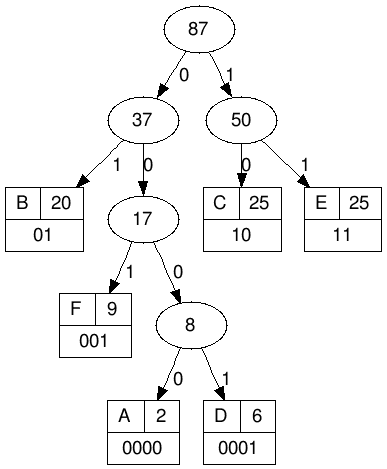
\includegraphics[scale=.5]{problem2.png}\\
		\item $B =01, C = 10, E = 11, F = 001, A = 0000, D = 0001$ \\
		\item 199 bits \\
		\item $.28$
	\end{enumerate}
		
		
	\newpage
	\noindent{\bf Solution for Problem 3}\\
	\begin{enumerate}
		\item 
		\begin{align}
			MW(i,j) &= \{\min\{MW(i-1,j),MW(i,j-1),MW(i-1,j-1)\} + w(i,j)\}\\
			prevm(i,j) &= \min\{(MW(i-1,j),MW(i,j-1),MW(i-1,j-1)\}\\
			C(i,j) &= [ prevm(i,j) = MW(i-1,j) ? C(i-1,j) : 0 ] +\\
			[ prevm(i,j) &= MW(i,j-1) ? C(i,j-1) : 0 ] +\\
			[ prevm(i,j) &= MW(i-1,j-1) ? C(i-1,j-1) : 0 ] \\
		\end{align}
		\item
		For every I and J compute MW and C saving them in tables starting at the end of the graph, then use the saved values to compute the next set of I and J working your way back to the origin of the table. The running time would be $\theta(M*N)$.		
	\end{enumerate}
	
	\noindent{\bf Solution for Problem 4}\\
	\noindent{\bf Algorithm 1 (Kruskal's Algorithm)}
	\begin{enumerate}
		\item Find the minimum spanning tree over a graph.
		\item 
		\begin{itemize}
			\item Create a forest F where each tree contains a single vertex.
			\item Create a set S containing all the edges in the graph.
			\item While is is nonempty and F does not cover every edge in the tree (is not spanning): remove an edge with the minimum weight from S, If that edge connects two different trees, then add it to the forest, combining two trees into a single tree, other wise discard that edge.
			\item When the loop is finished there will only be one item in F and that will be a minimum spanning tree.
		\end{itemize}
		\item This will work because of two facts, one that it will always produce a spanning tree. This can be shown because any cycles would have been avoided because the edge necessary to create a cycle would not be added because it would not not merge two trees in F, and because when ever a edge that does join two trees in F is encountered it is added used to merge two trees so there can be no disconnected trees in F. Second it can be shown that the tree will be minimal by induction using the fact the the first tree will always be minimum and any tree created using that tree can be made to be minimum using a greedy technique.
		\item \url{http://en.wikipedia.org/wiki/Kruskal%27s_algorithm}
	\end{enumerate}		
	\noindent{\bf Algorithm 2  (Malfattis Circles)}
	\begin{enumerate}
		\item Find three circle inside of a given triangle that are tangent to the other two circles and two side of the triangle.
		\item Inscribe a circle of maximal radius within the triangle, inscribe a circle in the largest of the three corners, then inscribe the last circle in the largest of the five remaining areas.
		\item This can be shown to work by going through all the possible cases of this problem and showing that the greedy algorithm with find an optimal solution. This was done by Zalgaller and Los' (1994).
		\item \url{http://en.wikipedia.org/wiki/Malfatti_circles}
	\end{enumerate}
	
	\noindent{\bf Solution for Problem 5} \\
	\noindent{\bf Algorithm 1 (Fibonacci sequence)}
	\begin{enumerate}
		\item Find the nth Fibonacci number
		\item The recursive solution will work for this in small cases but when the n gets large the amount of recursion required to successfully get the nth fibonacci number is massive and will almost surly cause a stack overflow, and be extremely slow.
		\item If dynamic programming is used this turns into an iterative problem and the same problem is never solved twice, this eliminates both the problem of it being slow and the stack overflow issue.
		\item \url{http://en.wikipedia.org/wiki/Dynamic_programming}
	\end{enumerate}
	
	\noindent{\bf Algorithm 2 (Sequence Alignment}
	\begin{enumerate}
		\item Find the set of edits which have the lowest cost that will transform the first sequence into the second.
		\item The recursive solution takes to much space and resolves the same problems to many times causing the algorithm to be slow.
		\item If dynamic programming is used the problem can be transformed into a matrix where you can select the optimum for the cells near where you are currently looking, this will take no extra space and the solutions with me memorized eliminating duplicated work.
		\item \url{http://en.wikipedia.org/wiki/Dynamic_programming}
	\end{enumerate}
\end{document}